\chapter{系统实现与测试}

本章将实现的PE文件虚拟机加壳和PE文件二进制混淆器组装成一个PE文件保护系统,并分别对本系统的保护壳和加密壳进行了功能验证、加密性能评估。其中本系统虚拟机壳的多样化Handler是在已有的虚拟机壳进行修改,并进行了Handler多样化的改进,增加了加壳后文件二进制编码的多样性,对逆向攻击者进行了有效的误导,二进制混淆器针对静态调试器进行防御,提出一种对函数间基本块交换的混淆算法,并记录交换块的索引放到文件的最后节表中,但由于交换函数间指令后修复程序的运行环境如内存、堆、栈、寄存器等难度太高,本文将针对MOV、SUB、ADD等不影响堆栈的指令进行交换,其余指令在保证能够恢复运行时的环境也可以实现,本章将会对以上的动态和静态保护措施进行实现和测试。


\section{总体设计方案}

\subsection{编程语言的选择}

通常情况下PE文件二进制保护软件使用C语言或者汇编来编写,市面流行的加密壳的外壳部分通常使用汇编代码,使用汇编语言编写,可以实现更加复杂的算法并且对PE文件的二进制混淆算法更容易实现,但是汇编语言难以掌握,并且通常情况下不具有可移植性,所以本保护系统将会使用C++和汇编语言编译器为X86nasm混合编程的方式,在需要对PE文件加壳的复杂位置使用汇编语言,程序的整体架构采用C++,这极大地提高了开发效率和降低了开发难度。

\subsection{软件的系统构架}

本系统采用模块化设计有利于系统的开发和维护,采用模块化结构有利于对软件功能进行细分,模块出现问题更利于修改。本系统有以下几个模块构成:外壳添加模块、反调试模块、特殊数据处理模块、区块压缩模块、输入表构建模块、反静态分析模块、虚拟机模块、PE文件读取模块组成。其中反调试模块、区块压缩模块、虚拟机模块采用汇编语言编写,采用X86nasm编译器。

\section{功能验证}

功能测试部分将对系统中的虚拟机加密和二进制混淆器的功能分别进行测试。在32位Windows 10系统下磁盘空间为120G、内存为2G的环境下进行功能测试,选择32位PE文件notepad.exe作为测试文件。在未进行虚拟机加密或未经二进制混淆之前,程序Aseprite.exe的运行情况如图\ref{aseprite}所示。

\begin{figure}[htbp]
	\centering
	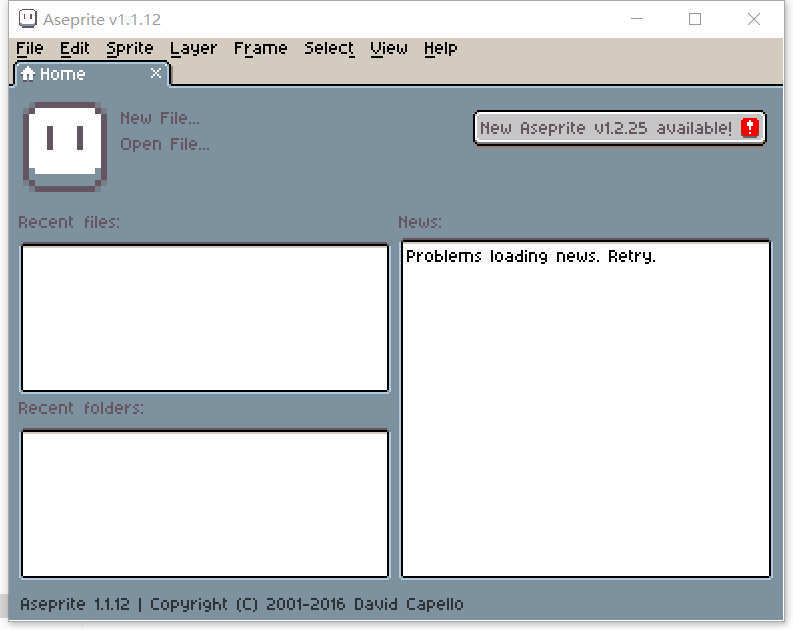
\includegraphics[width=10cm]{aseprite.png}
	\bicaption{程序Aseprite运行时}{When the program Aseprite is running}
	\label{aseprite}
\end{figure}

\subsection{虚拟机加壳功能验证}

加密壳由一个可执行文件aseprite.exe和一个加密脚本protect.bat组成。通过对脚本protect.bat调用虚拟机壳对aseprite.exe进行加壳的运行时如图\ref{aseprite},加密密钥为0x3275923A。



使用PEiD对aseprite进行加壳分析,加壳前节区如图\ref{jie},加壳后节区如图\ref{jiehou}。

\begin{figure}[htbp]
	\centering
	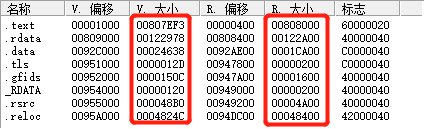
\includegraphics[width=10cm]{jie.png}
	\bicaption{Aseprite加壳前节表}{Aseprite Packing Front Section Table}
	\label{jie}
\end{figure}
\begin{figure}[htbp]
	\centering
	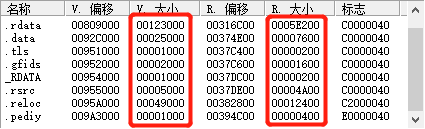
\includegraphics[width=10cm]{jiehou.png}
	\bicaption{Aseprite加壳后节表}{Aseprite packed back section table}
	\label{jiehou}
\end{figure}


通过对图\ref{jie}和图\ref{jiehou}中的红色框出数据分析,在加壳后,PE文件中的节表数据已经被修改, 并且添加了加壳用到的新节.pediy,此时大部分节表数据已经被压缩,成功添加了.pediy新节。
aseprite程序加壳后的运行时情况成功打开,与加壳功能一致,表明加壳成功。运行结果一致,加壳后的程序能够正常运行,表明加密壳的功能正常,能够对PE文件的有效加壳。


\subsection{二进制混淆器功能验证}

二进制混淆器只有一个可执行文件shell.exe,对文件Calculator.exe进行混淆,Calculator为Windows10中自带的计算器,下面通过查看Calculator.exe程序在混淆前后的函数间的调用变化在说明保护的有效性。使用二进制混淆器对Calculator加密后的运行情况如图\ref{jisuanqi}所示。

\begin{figure}[htbp]
	\centering
	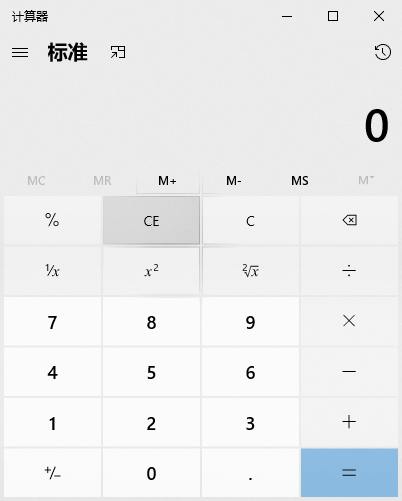
\includegraphics[width=6cm]{jisuanqi.png}
	\bicaption{Calculator.exe使用二进制混淆后的运行情况}{Operation of Calculator.exe after using binary obfuscation}
	\label{jisuanqi}
\end{figure}

计算器的功能正常运行,为了更深入的测试二进制混淆效果,下面使用IDA PRO对该程序进行反汇编,通过查看Calculator程序在混淆前后的函数控制流来观察加密的有效性。在加密前后Calculator的函数sub\_403339的控制流图分别如图\ref{403339}和图\ref{403339}所示,图中序号表示函数内部的基本块序号。
\begin{figure}[htbp]
	\centering
	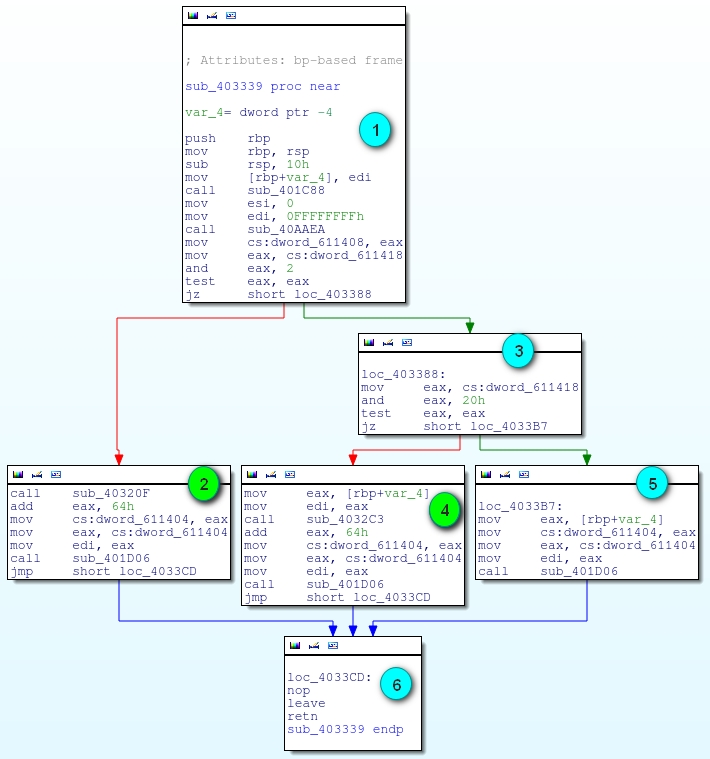
\includegraphics[width=14cm]{403339.jpg}
	\bicaption{加密前sub\_403339函数的控制流图IDA截图}{Control flow diagram of sub\_403339 function before encryption}
	\label{403339}
\end{figure}
\begin{figure}[htbp]
	\centering
	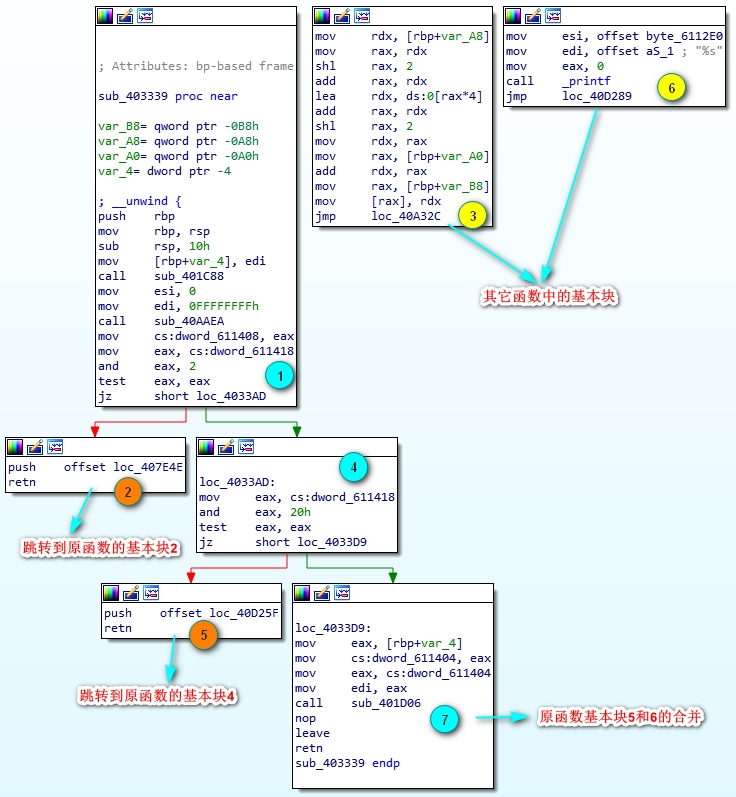
\includegraphics[width=14cm]{403339hou.jpg}
	\bicaption{加密后sub\_403339函数的控制流图IDA截图}{Control flow diagram of sub\_403339 function after encryption}
	\label{403339hou}
\end{figure}

由图\ref{403339}和图\ref{403339hou}可知,加密前后函数sub\_403339分别包含了6个和7个基本块。加密后,原函数的1和3基本块加密前后基本没有发生变化,分别对应加密后的1和4基本块;原函数中5和6基本块内容也没有变化,加密后被合成了基本块7;原函数中的2和4基本块被交换到了其他函数中;加密后函数中多了两个其他函数的3和6基本块,且基本块最后是一条jmp指令,通过该jmp指令将控制流转移到下一个基本块;原函数中对于基本块2和4的控制流转移通过基本块2和5中push+retn型指令实现。

加密后,参与加密函数内部的部分基本块被交换到了其他函数中,被交换的基本块通常有其他的函数的基本块,加大了使用IDA等静态分析器的分析难度,整个程序的控制流信息被打乱。

综上可知,二进制混淆器对程序进行加密后,原有的控制流信息得到了隐藏,达到了对PE文件加密的目的,二进制混淆器功能正常。

\section{性能评估}

性能评估在32位Windows10系统下,内存为2G,磁盘空间为60G下进行,评估内容包括静态混淆技术加密保护和虚拟机保护有效性。使用的测试样本为Windwos10下自带程序和目前流行软件。

\subsection{虚拟机加壳性能评估}

本节将对虚拟机加壳与流行加壳软件进行性能对比,其中包括压缩壳和加密壳,对比的变量为不同的测试程序,对比的输出数据为程序加壳后的大小、开启用时、和执行一次任务所用时间对比,通过计算得出压缩率、启动时间延迟百分比,额外运行时间开销百分比。

使用UPX软件这款压缩壳作为对照组。这里说明一下,使用UPX压缩壳软件作为对照组,是因为软件虚拟机加壳下,使用虚拟机加壳,相当于软件内置一个虚拟机解释器,在执行过程中采用边执行二进制代码边进行解释,程序的运行时间是最重要的性能指标,所以,在能保证程序正常运行的情况下,程序的运行时间是最重要的参考指标。至于加密壳,其运行时间远远小于虚拟机加壳,在这一方便,虚拟机加壳性能与加密壳性能差距太大, 所以不能作为对照组。尽管UPX是一个压缩壳,但是现在未公布的Windows压缩壳大部分是参考UPX进行修改,所以使用UPX作为加壳对照组具有一定意义。

% Please add the following required packages to your document preamble:
% \usepackage{multirow}
% Please add the following required packages to your document preamble:
% \usepackage{multirow}
\begin{table}[htbp]
	\centering
	\bicaption{测试程序加壳前后大小变化}{The size change of the test program before and after packing}
	\begin{tabular}{c|c|cc|cc}
		\bottomrule[1.5pt]
		\multirow{2}{*}{测试程序} & 原始程序   & \multicolumn{2}{c|}{UPX加壳后} & \multicolumn{2}{c}{加密壳加壳后} \\ \cline{2-6} 
		& 大小(KB) & 大小(KB)       & 压缩率(\%)      & 大小(KB)     & 额外空间开销(\%)     \\ \hline
		maps                  & 21     & 8            & 40.9         & 40         & 93.0           \\ \hline
		cacls                 & 33     & 8            & 26.9         & 45         & 38.7           \\ \hline
		mkdir                 & 72     & 32           & 45.7         & 110        & 54.0           \\ \hline
		bscmake               & 95     & 36           & 37.9         & 116        & 23.0           \\ \hline
		ls                    & 146    & 35           & 24.5         & 156        & 7.6            \\ \hline
		aseprite              & 3668   & 656          & 17.9         & 3851       & 0.5            \\ 
		\toprule[1.5pt]
	\end{tabular}

	\label{changesize}
\end{table}


从表\ref{changesize}可以看出,在测试程序大小小于100KB时,加壳导致的额外空间开销明显降低了,程序aseprite加壳后产生的额外空间开销甚至只有0.5$\%$。

% Please add the following required packages to your document preamble:
% \usepackage{multirow}
\begin{table}[htbp]
	\centering
			
	\bicaption{测试程序加壳前后时间变化}{Time changes before and after the test program is packed}
	\begin{tabular}{l|l|ll|ll}
		\bottomrule[1.5pt]
		\multirow{2}{*}{测试程序} & 原始程序 & \multicolumn{2}{l|}{UPX加壳后} & \multicolumn{2}{l}{加密壳加壳后} \\ \cline{2-6} 
		&
		\begin{tabular}[c]{@{}l@{}}平均运行\\ 时间(ms)\end{tabular} &
		\begin{tabular}[c]{@{}l@{}}平均运行\\ 时间(ms)\end{tabular} &
		\begin{tabular}[c]{@{}l@{}}额外时间\\ 开销(\%)\end{tabular} &
		\begin{tabular}[c]{@{}l@{}}平均运行\\ 时间(ms)\end{tabular} &
		\begin{tabular}[c]{@{}l@{}}额外时间\\ 开销(\%)\end{tabular} \\ \hline
		maps                  & 5    & 8           & 66.7\%        & 6            & 33.3         \\ \hline
		
		cacls                 & 120  & 127         & 6.2           & 131          & 9.8          \\ \hline
		mkdir                 & 44   & 47          & 8.1           & 51           & 16.3         \\ \hline
		bscmake               & 253  & 272         & 7.6           & 275          & 9.0          \\ \hline
		ls                    & 30   & 31          & 4.9           & 32           & 8.5          \\ \hline
		aseprite              & 540  & 561         & 3.9           & 564          & 4.5          \\
	    \toprule[1.5pt]
	\end{tabular}

	\label{changetime}
\end{table}
从表\ref{changetime}可以看出,使用本文加密壳加壳后的程序额外运行时间比较少,和UPX加壳软件加壳后产生的额外运行时间开销接近。时间开销相对不大的一个原因是加密壳只进行了函数间基本块的交换,使用随机算法,没有对程序汇编代码进行压缩,时间复杂度较低,如果需要对加密性能进行强化,可以使用更复杂或使用自定义的加密算法。所以,加密壳加壳后程序产生的额外时间和空间开销比较小,可以较好地满足实际应用。


\subsection{二进制混淆器功能评估}

本节通过二进制混淆器的指令执行效率进行评估来判断本文提出的混淆算法的有效性,评估的指标包括程序混淆后的混淆强度、运行时间开销、稳定性、隐蔽性。

为对比系统中混淆器的性能情况,使用市面上流行的二进制代码混淆工具Virbox Protector对程序混淆后的结果作为对照。

\subsubsection{混淆强度}

混淆强度的评估使用赵玉洁等提出的控制流循环复杂度和单条指令执行效率来度量。其中指令执行效率的公式为:$\mathit{IE = Id/Is}$,其中$\mathit{Is}$、$\mathit{Id}$分别表示被测试程序所包含的总指令数量和被测试程序中被运行过的指令数量;控制流循环复杂度的公式为:$\mathit{V(G)=e-n+2}$,其中e表示边的总数,n表示节点(基本块)的总数,测试程序经过混淆器混淆前后的指令执行率如表\ref{order}所示。

% Please add the following required packages to your document preamble:
% \usepackage{multirow}
\begin{table}[htbp]
	\centering
	\bicaption{混淆器混淆前后测试程序的指令执行率}{The instruction execution rate of the test program before and after obfuscation}
	\begin{tabular}{c|ccc|ccc}
		\bottomrule[1.5pt]
		\multirow{2}{*}{测试程序} & \multicolumn{3}{c|}{原始程序} & \multicolumn{3}{c}{混淆后程序} \\ \cline{2-7} 
		&
		\begin{tabular}[c]{@{}c@{}}静态指令\\ 数(条)\end{tabular} &
		\begin{tabular}[c]{@{}c@{}}动态指令\\ 数(条)\end{tabular} &
		\begin{tabular}[c]{@{}c@{}}执行率\\ (\%)\end{tabular} &
		\begin{tabular}[c]{@{}c@{}}静态指令\\ 数(条)\end{tabular} &
		\begin{tabular}[c]{@{}c@{}}动态指令\\ 数(条)\end{tabular} &
		\begin{tabular}[c]{@{}c@{}}执行率\\ (\%)\end{tabular} \\ \hline
		maps                  & 4755    & 1059   & 22.27  & 4899     & 1210   & 24.69  \\ \hline
		cacls                 & 3306    & 761    & 23.01  & 3514     & 810    & 23.05  \\ \hline
		mkdir                 & 21230   & 4097   & 19.29  & 22019    & 4600   & 20.89  \\ \hline
		bscmake               & 8185    & 1975   & 24.12  & 9100     & 2216   & 24.35  \\ \hline
		ls                    & 12523   & 2439   & 19.47  & 12699    & 3010   & 23.70  \\ \hline
		aseprite              & 193966  & 32374  & 16.68  & 196109   & 41409  & 21.11  \\
		\toprule[1.5pt]
	\end{tabular}

	\label{order}
\end{table}
程序在混淆之后,静态指令和动态指令都有所增加,这是因为采用了建立索引进行函数间基本块交换的混淆算法,在原有程序的基础上,增加了一些指令数据来实现函数间的跳转,虽然跳转的只是一些MOV、ADD、SUB等不影响寄存器和堆栈的指令,但是其指令数量还是有所提高,由原始程序和混淆程序的指令执行率可知,程序中每条执行被执行概率增加了,一定程序上反映出了程序的复杂性增加了。使用Virbox Protector混淆后程序的执行执行效率如表\ref{Virbox}。

\begin{table}[htbp]
	\centering
	\bicaption{Virbox Protector混淆后程序的指令执行率}{The instruction execution rate of the program after Virbox Protector confusion}
	\begin{tabular}{cccccc}
		\bottomrule[1.5pt]
		测试程序     & Ftotal & Fobf & 静态指令数  & 动态指令数 & 指令执行率 \\ \hline
		maps     & 126    & 14   & 4518   & 1198  & 26.51 \\
		cacls    & 39     & 7    & 3214   & 943   & 29.34 \\
		mkdir    & 234    & 15   & 14981  & 4709  & 31.43 \\
		bscmake  & 157    & 15   & 4910   & 1598  & 32.54 \\
		ls       & 164    & 14   & 46910  & 6102  & 13.00 \\
		aseprite & 6019   & 99   & 259838 & 34631 & 13.32 \\ 
		\toprule[1.5pt]
	\end{tabular}

	\label{Virbox}
\end{table}
其中FOBF、FTOTAL分别表示参与混淆的函数个数和程序的函数总数。从表\ref{Virbox} 可以看出几点:1.经过Virbox Protector混淆之后,不同程序的静态执行数量出现了增加和减少两种情况,这是Virbox Protector的混淆机制导致的,使用IDA Pro查看混淆后的程序的二进制汇编代码可知,在反汇编之后存在大量的数据,在静态反汇编时是以db指令存在的,被反汇编当做数据对待,但在执行时,其实在被解密后是以普通汇编指令执行的;2.当程序增加较多的静态指令数量时,程序的指令执行率未混淆之前甚至高于混淆之后,当增加较少的静态指令数量时,程序的执行效率比混淆前要高很多。所测试的程序指令执行率有减少也有增加,这是因为Virbox Protector内部使用了不同的混淆机制,本课题只使用一种,比如某些垃圾指令不被执行会降低程序的指令执行效率,而将一条会被执行的指令拆分成多条执行或添加被执行的垃圾执行会提高程序执行率。

测试程序在混淆前后控制流循环复杂度如表\ref{protector_2}所示。

\begin{table}[htbp]
	\centering
	\bicaption{混淆前后测试程序控制流循环复杂度}{Test program control flow loop complexity before and after confusion}
	\begin{tabular}{c|c|cc|cc}
		\bottomrule[1.5pt]
		\multirow{2}{*}{测试程序} & \multirow{2}{*}{原始复杂度} & \multicolumn{2}{c|}{Virbox Protector混淆后} & \multicolumn{2}{c}{混淆器混淆后} \\ \cline{3-6} 
		&       & 复杂度   & 增长率(\%) & 复杂度   & 增长率(\%) \\ \hline
		maps     & 267   & 184   & -31.1   & 279   & 4.49    \\
		cacls    & 318   & 123   & -61.3   & 329   & 3.45    \\
		mkdir    & 778   & 1690  & 117.2   & 920   & 18.25   \\
		bscmake  & 378   & 298   & -21.2   & 451   & 19.31   \\
		ls       & 934   & 3890  & 316.4   & 1090  & 16.70   \\
		aseprite & 34509 & 40109 & 16.2    & 37909 & 9.85    \\ 
		\toprule[1.5pt]
	\end{tabular}

	\label{protector_2}
\end{table}

使用Virbox Protector混淆后的程序的的控制流循环复杂度没有固定的规则,控制流循环复杂度有的数据特别高,有的甚至出现负数。而经过本课题的混淆器混淆之后,基本控制流的复杂度和增长率可以呈现一定的规律,程序的增长率基本维持在7$\%$-11$\%$,这说明在不考虑垃圾指令优化时,使用单种混淆方式通常情况下复杂度是增加的。

值得注意的是,Virbox Protector处理过后的程序的控制流循环复杂度降低了,但是并不代表程序的控制减少了,由于Virbox Protector包含多种混淆机制,在执行时有大量的数据需要解密后执行,所以程序的动态控制流会更复杂。

根据上述测试结果,可以得到二进制混淆器加密前后指令复杂性和控制流循环复杂度的变化以及与Virbox Protector软件的混淆结果对比,可以看到,经过二进制混淆器混淆后的程序的指令复杂度得到一定提高,表明混淆算法的混淆强度指标合格。同时也反映出了通过指令的执行率和控制流循环夫再度来衡量代码混淆程序的局限性。

\subsubsection{运行时间开销的对比}


二进制混淆器和Virbox Protector对测试程序混淆后,程序的运行时间开销的对比如表\ref{shijianhunxiao}


\begin{table}[htbp]
	\centering
	\bicaption{混淆后测试程序的额外开销}{Additional overhead of test program after obfuscation}
	\begin{tabular}{c|cc|cccc}
		\bottomrule[1.5pt]
		\multirow{2}{*}{测试程序} & \multicolumn{2}{c|}{原始程序} & \multicolumn{2}{c}{混淆器混淆后}      & \multicolumn{2}{c}{额外开销} \\ \cline{2-7} 
		&
		大小(KB) &
		\begin{tabular}[c]{@{}c@{}}平均运行\\ 时间(ms)\end{tabular} &
		大小(KB) &
		\multicolumn{1}{c|}{\begin{tabular}[c]{@{}c@{}}平均运行\\ 时间(ms)\end{tabular}} &
		\begin{tabular}[c]{@{}c@{}}空间\\ (\%)\end{tabular} &
		\begin{tabular}[c]{@{}c@{}}时间\\ (\%)\end{tabular} \\ \hline
		maps                  & 40           & 3          & 43   & \multicolumn{1}{c|}{5}   & 7.5         & 66.7       \\ \hline
		cacls                 & 78           & 157        & 85   & \multicolumn{1}{c|}{170} & 8.9         & 8.2        \\ \hline
		mkdir                 & 124          & 223        & 130  & \multicolumn{1}{c|}{131} & 5.6         & 5.6        \\ \hline
		bscmake               & 68           & 28         & 72   & \multicolumn{1}{c|}{32}  & 5.8         & 14.2       \\ \hline
		ls                    & 120          & 91         & 128  & \multicolumn{1}{c|}{101} & 6.7         & 10.9       \\ \hline
		aseprite              & 5093         & 450        & 5609 & \multicolumn{1}{c|}{480} & 10.1        & 6.7        \\ 
		\toprule[1.5pt]
	\end{tabular}

 	\label{shijianhunxiao}
\end{table}

使用二进制混淆器后,程序的额外占用空间随着程序的占用空间增大而增大,空间开销在程序小于5M时空间开销低于10$\%$;程序的额外运行时间开销随着运行时间增加比例大约在8$\%$左右。由以上可得,二进制混淆器产生的额外开销所占比率并不高。由表\ref{ewaikaixiao}可知,

\begin{table}[htbp]
	\centering
	\bicaption{Virbox Protector混淆后测试程序的额外开销}{The extra cost of the test program after Virbox Protector obfuscation}
	\begin{tabular}{ccccc}
		\bottomrule[1.5pt]
		测试程序     & 大小(KB) & 空间开销(倍) & 时间(ms) & 时间开销(倍) \\ \hline
		maps     & 484    & 11.0    & 10.3   & 3.44    \\
		cacls    & 1723.8 & 22.1    & 282.6  & 1.8     \\
		mkdir    & 1277.2 & 10.3    & 691.3  & 3.10    \\
		bscmake  & 632.4  & 9.3     & 81.4   & 2.91    \\
		ls       & 588    & 4.9     & 171.9  & 1.89    \\
		aseprite & 6111.6 & 1.2     & 49.5   & 1.10    \\ 
		\toprule[1.5pt]
	\end{tabular}

	\label{ewaikaixiao}
\end{table}

使用Virbox Protector混淆后的程序的占用空间和运行时间开销都很高,这样会程序在实际使用起来的体验不如本课题的二进制混淆器。

\subsubsection{隐蔽性}

本课题隐蔽性通过计算经过二进制混淆前后的文件相似度来判断。 测试样本的混淆前后文件相似度使用radare中的radiff2工具来计算,经过混淆前后的相似度如表\ref{protector_2}所示。使用Virbox Protector加密过的程序的变化非常明显,可以很明确看出程序是经过混淆处理的,这样的程序隐蔽性较低。


\begin{table}[htbp]
	\centering
	\bicaption{混淆前后程序的相似度}{Program similarity before and after confusion}

	\begin{tabular}{c|c|c|c|c|c|c}
		\bottomrule[1.5pt]
		测试程序      & maps & cacls & mkdir & bscmake & ls & aseprite \\ \hline
		相似度(\%)   & 91   & 93    & 95    & 92      & 93 & 92       \\ \hline
		平均相似度(\%) & \multicolumn{6}{c}{93}                        \\ 
		\toprule[1.5pt]
	\end{tabular}
	\label{xiangsidu}
\end{table}

由表\ref{xiangsidu}可知,混淆前后,程序的相似度比较高,都在80$\%$以上,平均相似度为89$\%$。从上面可以得出,使用本课题的虚拟机的混淆程序不易被发现该程序是经过混淆的,这样降低了程序被逆向的风险,所以具有一定的抗逆向意义。

二进制混淆器与Virbox Protector对比,本文设计的二进制混淆器的混淆强度较低,同时在被逆向的情况下,本课题的保护壳更容易被成功逆向破解,这是因为本混淆器只实现了普通汇编指令如MOV、SUB、ADD等不影响寄存器和堆栈空间的指令的交换和混淆,如果将所有汇编指令都实现交换和混淆,产生的二进制混淆器的混淆强度将会高出一个级别。但是本文的二进制混淆器的运行时间、占用磁盘空间和隐蔽性能比较良好。

综上可知,加密后的程序的运行时间、磁盘占用空间和隐蔽性都要优于Virbox Protector,具有较好的实用性。这表明本文二进制混淆器的抵抗静态分析的能力较强,但是抵御动态分析方面存在不足。由上文可知,本混淆器可以与其他加壳工具兼容,实现混用,本文的二进制混淆器与其他保护壳共同使用时,可以产生较高的保护力。由此表明本文所提出的二进制混淆算法可以提高软件的抗逆向性能。

\section{本章小结}

本章首先对系统的实现和所选择的测试环境进行介绍,然后分别对虚拟机加壳器和二进制混淆器的功能进行了验证和性能进行评估,由实验结果可知,加壳器和二进制混淆器的功能正常、性能评估结果表明使用上述保护方法对二进制可执行程序进行保护具有一定实用性,总体实验结果表明所提出的虚拟机加壳方法和二进制混淆器组成的保护系统能够有效增强Windows下可执行程序的抗逆向能力。



















